
\section{Resolución}
\subsection{Organización}
Organización temporal y de trabajo

\subsection{Desarrollo}
Desarrollo y resolucion completa

\subsubsection{Entrenamiento}
En esta fase del KDD, se eligieron y entrenaron diferentes modelos matemáticos para el análisis del set de datos. El objetivo del proyecto es conseguir predecir las etiquetas de las señales de sonidos no verbales, para ello se entrenaron los siguientes modelos:
\begin{itemize}
    \item K-vecinos más cercanos (KNN)
    \item Redes de neuronas artificiales secuenciales (SNN)
\end{itemize}
Ambos algoritmos son supervisados, para la clasificación de datos nuevos se entrena al modelo con datos etiquetados y el modelo aprende en función de si ha clasificado bien o mal datos etiquetados.

La idea básica detrás de KNN es que los puntos de datos similares tienden a agruparse en el espacio de características. Cuando se clasifica un nuevo punto de datos (en este caso, un nuevo audio), el algoritmo busca los "K" puntos de datos más cercanos (vecinos) en el espacio de características. Luego, asigna la clase más común entre esos vecinos al punto de datos de prueba.

Para KNN se obtuvieron resultados poco satisfactorios con precisiones bajas. Aunque es posible que se pudieran obtener mejores resultados, utilizando representaciones de los datos como espectrogramas basados en los coeficientes cepstrales de Mel, se tomó la decisión de abordar el problema de clasificación principalmente con redes neuronales artificiales.

Las redes neuronales en el contexto del aprendizaje automático (machine learning) son un tipo de modelo computacional inspirado en la estructura y el funcionamiento del cerebro humano. Están compuestas por unidades de procesamiento llamadas neuronas artificiales que están organizadas en capas y conectadas mediante conexiones ponderadas.

Las redes neuronales articificiales o redes neuronales secuenciales (en adelante RNA), son excelentes en la clasificación de sonidos por ser capaces de aprender características complejas de los datos, su flexibilidad en la representación de datos y adaptabilidad, esto las convierte en clasificadores consistentes aprueba de fallos como pueden ser incompletitudes en los datos.

Se comenzó realizando arquitecturas secuenciales con capas densas. Este tipo de capas tienen la desventaja de que estudian de manera parcial el orden en el que aparencen los datos, y los sonidos que se pretenden estudiar tienen carácteristicas que son temporalmente dependientes, como puede ser tras una tos un sonido de inspiración o la variación en amplitud al final de la misma. Se probaron modelos más simples pocas capas y más complejos con muchas capas.



\begin{center}
    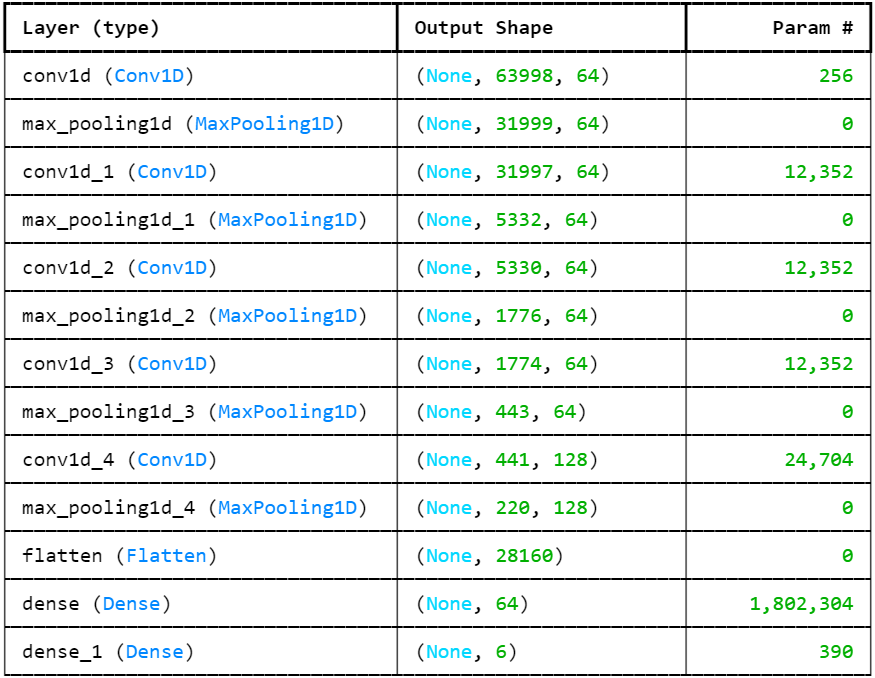
\includegraphics[width=0.8\textwidth]{ImagenesLatex/Conv1D_capas.PNG}
\end{center}


